\chapter{Benutzerdokumentation}

%\renewcommand{}{}

\section{Notation}

\begin{tabular}{l|l}
	Strg & die Steuerungstaste (Strg oder Ctrl) \\
	Shift & die Gro\ss schreibtaste (Shift) \\
	Alt & die Alt-Taste \\
	\\
	LMT & linke Mausetaste \\
	MMT & mittlere Maustaste \\
	RMT & rechte Maustaste \\
	MR & Mausrad\\
	\\
	Taste1 + Taste2 & hierbei sollen beide Tasten gleichzeitig gedr"uckt werden \\
\end{tabular}

\section{Installation}

\begin{figure}[htb]
\centering
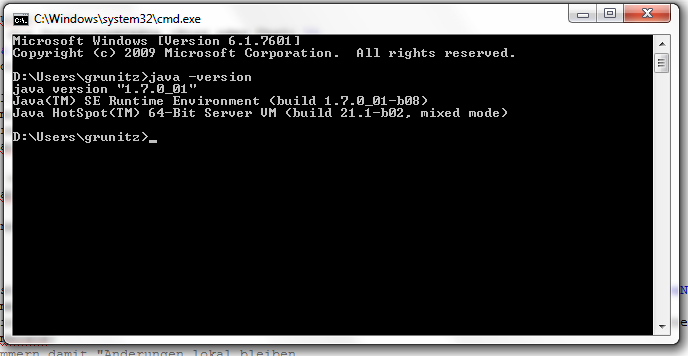
\includegraphics[width=0.8\textwidth]{bilder/java_version.png}
\caption{Kommandokonsole zeigt die installierte \javaNS-Version an}
\label{pic:java_version}
\end{figure}

Vor der Installation m"ussen sie sicherstellen, dass f"ur ihr Betriebssystem die aktuelle \javaNS-Version installiert ist.
Das Programm ben"otigt die Version \unit{1.7.0\_01} oder h"oher.
Um unter Windows die Versionsnummer ihrer \javaNS-Installation herauszufinden, f"uhren sie bitte folgende Schritte aus:
\begin{enumerate}
	{% Klammern damit "Anderungen lokal bleiben
	\renewcommand{\theenumi}{\arabic{enumi}}
	\renewcommand{\labelenumi}{{\theenumi}.}
	\item Dr"ucken sie die Windowstaste und \code{R} gleichzeitig.
	\item In dem neu ge"offneten Dialog geben sie den Befehl \code{cmd} ein und best"atigen ihn mit der Entertaste.
	\item Es hat sich nun eine Kommandokonsole ge"offnet. Geben sie dort den Befehl \code{java -version} ein.
	\item In der ersten Zeile steht ihre installierte \javaNS-Version. Das Fenster sollte dem in \picref{java_version} "ahneln.
	}
\end{enumerate}
Die Installation ist durch einfaches Kopieren des Programmverzeichnisses in ein beliebiges Verzeichnis auf ihrem Computer vollzogen.

\section{Starten des Programms}

\begin{figure}[htb]
\centering
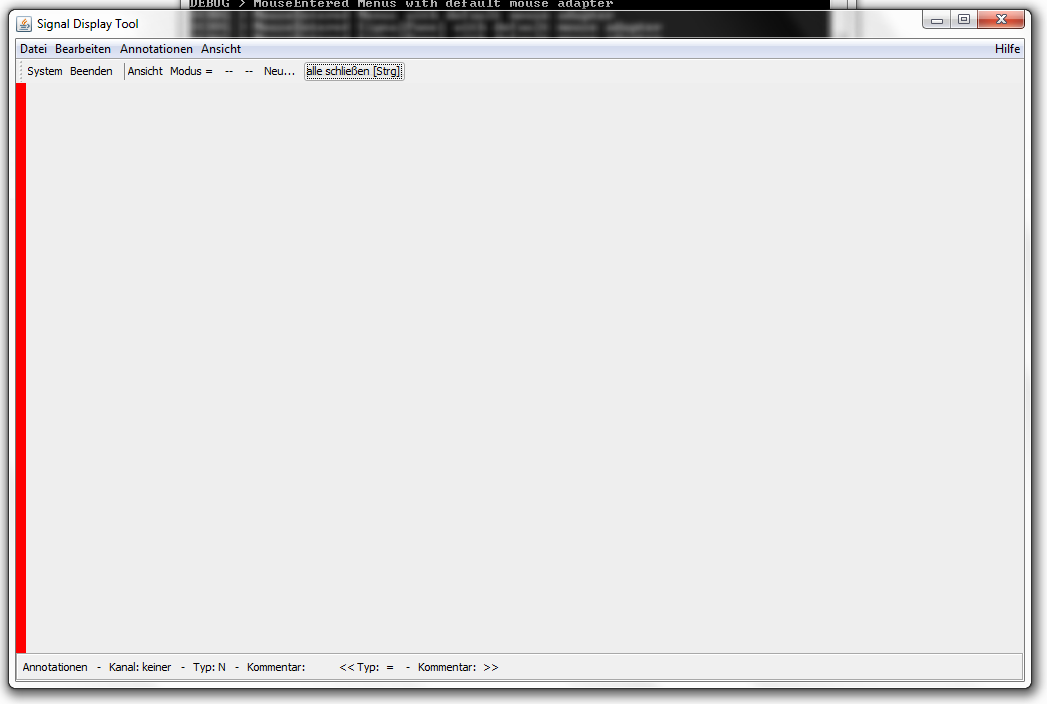
\includegraphics[width=\textwidth]{bilder/window.png}
\caption{Ansicht des Programms nach dem Start}
\label{pic:program_start}
\end{figure}

Wenn alle Dateien im richtigen Ordner sind kann das Programm durch einen Doppelklick auf die Datei \verb|Sigano.cmd| gestartet werden.
Es sollten sich dann zwei Fenster "offnen.
Das Fenster in dem nur Text steht kann getrost ignoriert werden, da dort nur Informationen f"ur den Entwickler ausgegeben werden.
Das Programmfenster sieht ungef"ahr so wie in \picref{program_start} dargestellt aus.

\section{Allgemeine Bedienung}

\begin{figure}[htb]
\centering
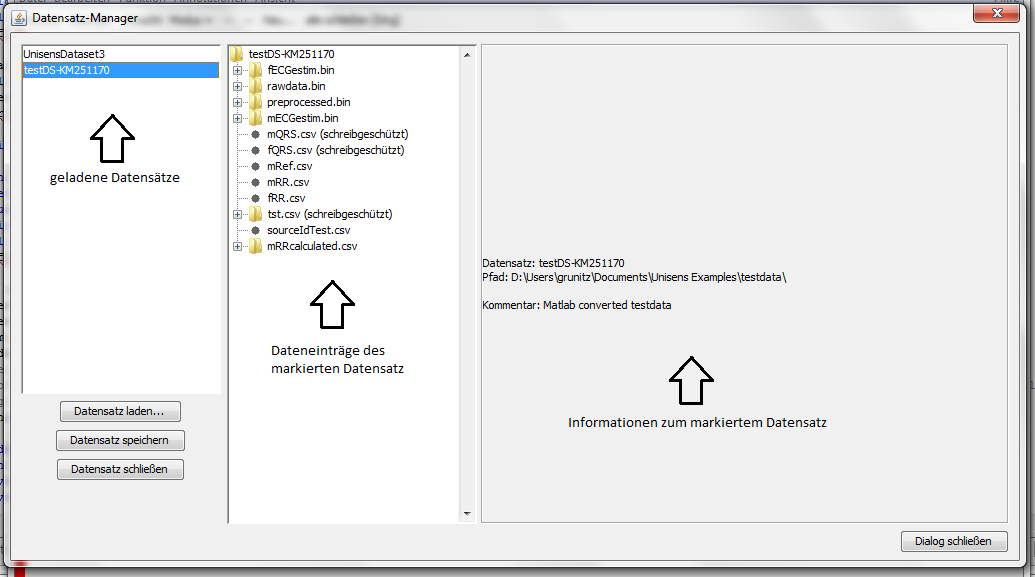
\includegraphics[width=\textwidth]{bilder/datensatzmanager.png}
\caption{Datensatzmanager zum Laden, Speichern und Schlie{\ss}en von Datens"atzen}
\label{pic:datensatzmanager}
\end{figure}

"Uber den Menueintrag \textsf{Datei - Datens"atze...} "offnet man den Datensatzmanagerdialog (siehe \picref{datensatzmanager}).
In diesem Dialog kann man Datens"atze mithilfe der Schaltfl"achen laden, speichern und schlie{\ss}en.
Geladen wird ein Datensatz "uber die Schaltfl"ache \textsf{Datensatz laden...}
In dem neue ge"offneten Dialog w"ahlt man den entsprechenden Ordner und dann die Datei \verb|unisens.xml| aus.
Wenn der Datensatz geladen wurde kann der Datensatzmanager geschlossen werden.
"Uber die Schaltfl"ache \textsf{Neu...} in der Toolbar kann eine neue Signalansicht ge"offnet werden.
In dem Dialog kann man mehrere Datenkan"ale (durch halten der \verb|Strg| Taste) ausgew"ahlt werden, die in der Signalansicht angezeigt werden sollen.
%Es werden dann alle in dem Datensatz vorhandenen Signale in einem eigenem Diagramm dargestellt.
%Bleibt das Fenster nach dem Laden grau aber es erscheint unter dem Mauszeiger ein gr"uner Streifen, dann sind zuviel Signale dargestellt.
Eine gr"une Markierung hebt die Signalansicht hervor, f"ur welches die aktuelle Maus- und Tastatureingabe gilt.
Folgende Tastebefehle stehen zur Verf"ugung:

\noindent
\begin{tabular}{c|l}
	\verb|Q| & schlie\ss t die ausgew"ahlte Signalansicht \\ \hline
	\verb|E| & "offnet den Signalauswahldialog: die markierten Signale werden in die\\
			 & Ansicht "ubernommen; mehrere Signale k"onnen mit \verb|Strg + LMT|\\
			 & ausgew"ahlt werden\\ \hline
	\verb|L| & blendet eine Legende ein\\ \hline
	\verb|MR| & bewegt das Signal entlang der Zeitachse\\ \hline
	\verb|Shift| + \verb|MR| & zoomt das Signal herein und heraus\\\hline
	\verb|MMT| & zentriert die Signalansichten auf den angeklickten Zeitpunkt\\
\end{tabular}

\section{Annotationen}

Annotationen werden als blaue Striche in den Signalverl"aufen dargestellt.
Um Annotationen setzen zu k"onnen, muss man als erstes einen (Annotations-)Kanal ausw"ahlen.
Das kann man "uber den Menupunkt \textsf{Annotationen - Kanal ausw"ahlen ...}.
Man kann aber auch einen neuen Kanal daf"ur anlegen "uber den Menupunkt \textsf{Annotationen - Kanal hinzuf"ugen ...}
In beiden F"allen muss man zuerst einen Datensatz ausw"ahlen und als n"achstes den Annotationskanal bestimmen/benennen.
Der gerade ausgw"ahlte Kanal ist unten in der Statusleiste angegeben.
Um Verwirrungen zu vermeiden sollte man immer sicher gehen, dass auch der ausgw"ahlte Annotationskanal im aktuell betrachtetem Diagramm auch dargestellt wird.

Annotationen k"onnen einfach durch dr"ucken der \verb|LMT| gesetzt werden.
Gel"oscht werden sie durch die Bet"atigung von \verb|Strg + LMT|.
Mit dem Halten der \verb|Shift|-Taste w"ahrend man die \verb|LMT| bet"atigt, kann man die Annotation, die man setzen m"ochte, editieren.
Im ersten Feld wird der Annotationstyp (N, B, V, ...) bestimmt und im zweiten Feld kann ein optionales Kommentar geschrieben werden.
Die Information "uber den Typ und den Kommentar der zu setzenden Annotation wird auch unten in der Statusleiste neben dem gew"ahlten Kanal angezeigt.
"Uber die Tasten \verb|1| bis \verb|4| kann man vordefiniert Annotationen ausw"ahlen:

\noindent
\begin{tabular}{c|c|l}
	\textbf{Ziffer} & \textbf{Typ} & \textbf{Kommentar} \\ \hline
	\verb|1| & N & keins \\
	\verb|2| & V & keins \\
	\verb|3| & B & signal loss\\
	\verb|4| & E & signal recovered\\
\end{tabular}

Informationen "uber die die Annotationen die sich gerade unter dem Mauszeiger befinden werden auch in der Statusleiste angezeigt.
Sie befinden sich am Ende der Leiste und sind mit "< und "> umklammert.

Um die gesamten "Anderungen zu speichern muss man \textsf{Datei - alles speichern} im Menu ausw"ahlen.

\section{Ansichten}

Um eine neue Signalansicht zu "offnen, muss man nur den Schalter \textsf{Neu ...} unter der Menuleiste bet"atigen.
Nachdem man die darzustellenden Signale ausgew"ahlt hat, wird die neue Ansicht am unteren Ende aller Signale dargestellt.
Wenn man alle Ansichten schlie\ss en m"ochte, kann man den Schalter \textsf{alle schlie\ss en} bei gedr"uckter \verb|Strg|-Taste dr"ucken.

Das Programm kennt drei verschiedene Anzeigemodi:
\begin{itemize}
	\item alle Signalansichten sind gleich hoch (Modus \verb|=|)
	\item eine Signalansicht ist gro\ss dargestellt und alle anderen teilen sich den verbleibenden Platz (Modus \verb|1|)
	\item zwei SignalAnsichten sind vergr"o\ss ert dargestellt und die restlichen teilen sich den restlichen Raum (Modus \verb|2|)
\end{itemize}
Mit den Schaltern rechts neben dem f"ur den Anzeigemodus kann man das/die Vergr"o\ss erungsauswahl ver"andern.
